%*****************************************
\chapter*{Résumé étendu}
\label{chap:resume-etendu}
%*****************************************

\section*{Contexte et motivation}
\label{sec:contexte-et-motivation}

Les solveurs SMT (\emph{Satisfiabilité modulo théories}) \cite{cvc5,verit} se sont imposés comme des outils centraux de la vérification formelle moderne.
Ces solveurs sont utilisés comme des outils pour la démonstration automatique de théorèmes qui intègrent le raisonnement propositionnel enrichies par des théories comme l’arithmétique linéaire, les fonctions non interprétées, ou encore les bit-vectors.
Leur grande efficacité en fait des composants essentiels de nombreux logiciels industriels et académiques, par exemple pour la modélisation et la vérification de systèmes critiques, la vérification de programmes et de matériels, l’analyse statique, ou encore l’intégration dans des assistants de preuve \cite{smtcoq,lean-smt}.

Cependant, cette efficacité s’accompagne d’une question fondamentale de confiance sur les résultats produits.
Les solveurs SMT sont des logiciels complexes, optimisés, et en évolution rapide.
Ils sont en outre souvent écrits en C/C++ pour des raisons de performance, ce qui complique fortement leur vérification formelle et leur formalisation.
Il est donc difficile d’en certifier entièrement l’implémentation, et l’expérience montre que des bogues peuvent conduire à des verdicts incorrects \cite{bugsmt}.
Dans des contextes critiques, où leur résultat entraîne une décision de sûreté, il devient indispensable de renforcer notre confiance dans ces outils.

Une approche prometteuse consiste à certifier non pas l'implémentation du solveur, mais ses résultats, via la technique du \emph{proof logging}\cite{acmsmt}.
Cette approche consiste à ce que le solveur produise ainsi une trace de preuve appelée \emph{certificat}, qui justifie le verdict.
Un outil indépendant, plus simple que le solveur, vérifie ensuite ce certificat.
Cette séparation des rôles est attrayante car la vérification d’une preuve est conceptuellement plus simple et peut s’appuyer sur un noyau de confiance réduit.

\begin{figure}[b]
    \centering
    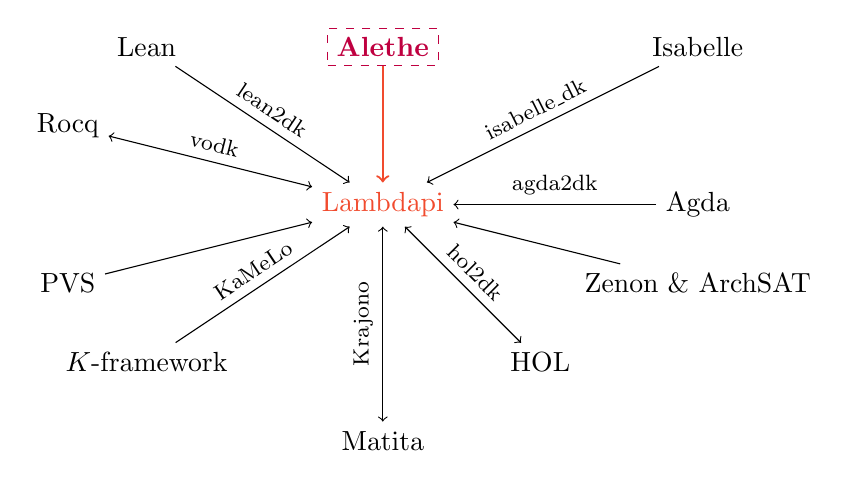
\begin{tikzpicture}
      \path (0,0) node (lp) {\textcolor{RedOrange}{Lambdapi}}
            (-4,1) node (coq) {Rocq}
            (-3,2) node (lean) {Lean}
            (0,2) node [draw, dashed, purple] (smt) {\color{purple}\textbf{Alethe}}
            (4,2) node (isa) {Isabelle}
            (4,0) node (agda) {Agda}
            (-3,-2) node (k) {$\mathbb{K}$-framework}
            (0,-3) node (mat) {Matita}
            (2,-2) node (hol) {HOL}
            (-4,-1) node (pvs) {PVS}
            (4,-1) node (ze) {Zenon \& ArchSAT}
            ;
      \draw[->,RedOrange, thick] (smt) -- (lp) node[midway,sloped,above] {};
      \draw[->] (lean) -- (lp) node[midway,sloped,above] {\footnotesize{lean2dk}};
      \draw[->] (isa) -- (lp) node[midway,sloped,above] {\footnotesize{isabelle\_dk}};
      \draw[->] (agda) -- (lp) node[midway,sloped,above] {\footnotesize{agda2dk}};
      \draw[->] (ze) -- (lp) node[midway,sloped,above] {};
      \draw[<->] (hol) -- (lp) node[midway,sloped,above] {\footnotesize{hol2dk}};
      \draw[<->] (mat) -- (lp) node[midway,sloped,above] {\footnotesize{Krajono}};
      \draw[->] (pvs) -- (lp);
      \draw[->] (k) -- (lp) node[midway,sloped,above] {\footnotesize{KaMeLo}};
      \draw[<->] (coq) -- (lp)  node[midway,sloped,above] {\footnotesize{vodk}};
    \end{tikzpicture}
    \captionsetup{list=no}
    \caption{Lambdapi, un langage assembleur pour les systèmes de preuve.}
    \label{fig:fr-interop-intro}
\end{figure}

Le format de preuve Alethe \cite{alethe} a émergé comme un format de preuve standard pour représenter des preuves d’insatisfiabilité SMT.
Alethe repose sur la SMT-LIB \cite{smtlib}. Les preuves sont organisées comme une suite d’étapes, et Alethe propose un catalogue de règles de raisonnement couvrant la résolution, des lemmes de théorie, des simplifications, les quantificateurs et la skolémisation. 
Néanmoins, Alethe ne dispose pas encore d’un vérificateur certifié largement adopté, ce qui limite son rôle comme format d’échange réellement fiable \cite{carcara}.

Cette thèse répond à ce besoin en développant un cadre de \emph{reconstruction} de preuves Alethe dans Lambdapi \cite{lambdapi}.
Lambdapi est un assistant de preuve fondé sur le $\lambda\Pi$-calcul modulo théories, conçu comme un langage pivot pour échanger des preuves entre systèmes.
Comme l’illustre la \Cref{fig:fr-interop-intro}, de nombreux assistants et outils peuvent exporter ou importer des preuves via Lambdapi, qui joue alors le rôle de ``langage assembleur'' pour les systèmes de preuve.
Reconstruire une preuve Alethe dans Lambdapi revient à produire un terme de preuve dont la validité est vérifiée par le noyau de Lambdapi, ce qui fournit une garantie forte.
L’objectif est ainsi de rendre les preuves Alethe portables et vérifiables indépendamment du solveur.


\section*{Alethe, preuves SMT et enjeux de vérification}

Le format de traces de preuve Alethe \cite{alethespec} pour les solveurs SMT se compose de deux parties :
un langage de traces fondé sur SMT-LIB, et une collection de règles de preuve.
Les traces constituent des témoins d’insatisfiabilité d’un ensemble de contraintes.
Elles prennent la forme de séquences $a_1 \dots a_m~t_1 \dots t_n$ où les $a_i$ correspondent aux contraintes du problème SMT initial réfuté, chaque $t_i$ est une clause inférée à partir des éléments précédents de la séquence, et $t_n$ est $\bot$ i.e. la clause vide.
Dans la suite, nous désignons le problème SMT-LIB comme le \emph{problème d’entrée}.

\begin{lstlisting}[language=SMT]
(set-logic UF)
(declare-sort U 0)
(declare-fun a () U)
(declare-fun b () U)
(declare-fun p (U) Bool)
(assert (p a))
(assert (= a b))
(assert (not (p b)))
(check-sat)
(get-proof)
\end{lstlisting}

\begin{center}
$\lightning$
\end{center}

\begin{lstlisting}[language=SMT,caption={Un problème SMT et sa preuve Alethe trouvée par cvc5.},label={lst:fr-smtexampleinput-fol},nolol]
(assume a0 (p a))
(assume a1 (= a b))
(assume a2 (not (p b)))
(step t1 (cl (not (= (p a) (p b))) (not (p a)) (p b)) :rule equiv_pos2)
(step t2 (cl (= (p a) (p b))) :rule cong :premises (a1))
(step t3 (cl (p b)) :rule resolution :premises (t1 t2 a0))
(step t4 (cl) :rule resolution :premises (a2 t3))
\end{lstlisting}

L’exemple de la \cref{lst:fr-smtexampleinput-fol} illustre ce principe : à partir du problème d’entrée, le solveur produit une trace Alethe composée d’étapes \kw{assume} et \kw{step}, aboutissant à la clause vide \kw{(cl)}.
Les solveurs SMT procèdent par réfutation : ils ajoutent $\neg p(b)$ aux hypothèses et prouvent l’\emph{insatisfiabilité}.
L’insatisfiabilité obtenue constitue alors un certificat de la validité de l’entaillement, dont le solveur fournit une preuve sous la forme d’une trace Alethe.

\renewcommand{\eqnhighlightshade}{35}

\begin{equation}
\label{eq:fr-step}
\tag{\textcolor{purple}{1}}
\eqnmarkbox[midpurple]{node2}{i}. \quad \eqnmarkbox[RoyalBlue]{node1}{\Gamma} ~\triangleright~ \eqnmarkbox[Emerald]{node3}{l_1 \dots l_n} \quad (\eqnmarkbox[rxpurple2]{node4}{\mathcal{R}}~\eqnmarkbox[darkpurple]{node5}{p_1 \dots p_m})~\eqnmarkbox[rxpink]{node6}{[a_1 \dots a_r]}
\annotate[yshift=-0.5em]{below, left}{node2}{indèxe}
\annotate[yshift=-0.5em]{below, right}{node1}{contexte}
\annotate[yshift=0.5em]{above, left}{node3}{clause}
\annotate[yshift=-0.5em]{below, right}{node4}{règle}
\annotate[yshift=-0.5em]{below, right}{node5}{prémisses}
\annotate[yshift=-0.5em]{below, right}{node6}{arguments}
\end{equation}

\bigskip\bigskip

Pour analyser et reconstruire de telles traces, nous décrivons maintenant la structure générale d’une étape Alethe, résumée en \cref{eq:fr-step}.
Une étape est constituée d’un indice \colorbox{midpurple!30}{$i$} $\in \mathbb{I}$, où $\mathbb{I}$ est un ensemble infini dénombrable d’indices (par exemple \kw{a0}, \kw{t1}), et d’une clause de formules \colorbox{Emerald!30}{$l_1, \dots, l_n$} représentant une disjonction $n$-aire.
Les étapes qui ne sont pas des hypothèses sont justifiées par une règle de preuve \colorbox{rxpurple2!30}{$\mathcal{R}$} qui dépend d’un ensemble éventuellement vide de prémisses $\{\colorbox{darkpurple!30}{$p_1 \dots p_m$}\} \subseteq \mathbb{I}$,
ne référant que des étapes antérieures, de sorte que la preuve forme un graphe orienté acyclique.
Une règle peut aussi dépendre d’une liste d’arguments \colorbox{rxpink!30}{$[a_1 \dots a_r]$}, où chaque argument $a_i$ est soit un terme, soit une paire $(x_i, t_i)$, où $x_i$ est une variable et $t_i$ un terme.
L’interprétation des arguments dépend de la règle.
Le contexte \colorbox{RoyalBlue!30}{$\Gamma$} d’une étape est une liste $c_1 \dots c_l$, où chaque élément $c_j$ est soit une variable, soit un couple variable-terme noté $x_j \mapsto t_j$.
Ainsi, les étapes dont le contexte est non vide contiennent des variables $x_j$ qui apparaissent dans \colorbox{Emerald!30}{$l_i$} et seront substituées par les $t_j$.
Les règles de preuve \colorbox{rxpurple2!30}{$\mathcal{R}$} incluent des lemmes de théorie et d'autre règle de logique comme la règle \kw{resolution}, qui correspond à l’hyper-résolution sur des clauses.

Ces éléments suffisent pour appréhender la preuve du \cref{lst:fr-smtexampleinput-fol}, qui comporte ici sept étapes.
Elle commence par trois premières étapes \kw{assume} (\kw{a0}, \kw{a1}, \kw{a2}) qui réaffirment les assertions du problème d’entrée.
Dans la syntaxe concrète, les étapes \kw{assume} disposent d’une commande dédiée \smtinline{assume}, afin de les distinguer clairement des étapes ordinaires, qui utilisent la commande \smtinline{step}.
Cette commande est du sucre syntaxique pour une commande \kw{step} utilisant la règle Alethe \kw{hole} qui admet une clause.
L’étape \kw{t1} introduit une tautologie de la forme $\neg (\varphi_1 \approx \varphi_2) \lor \neg \varphi_1 \lor \varphi_2$, justifiée par la règle \colorbox{rxpurple2!30}{\kw{equiv\_pos2}}.
L’étape \kw{t2} établit $p(a) \approx p(b)$ par congruence à partir de l’hypothèse \kw{a1} et matéralisée par la règle \colorbox{rxpurple2!30}{\kw{cong}}.
L’étape \kw{t3} applique ensuite la règle \colorbox{rxpurple2!30}{\kw{resolution}} aux prémisses \kw{t1}, \kw{t2} et \kw{a0} pour dériver $p(b)$.
Enfin, l’étape \kw{t4} conclut la preuve en produisant la clause vide i.e. $\bot$, concrètement notée \kw{(cl)}.
Remarquons que les contextes \colorbox{RoyalBlue!30}{$\Gamma$} de toutes les étapes sont vides dans cet exemple.

\subsection*{Preuve à forte granularité}
\label{ssec:fr-preuve-coarse-grained}


\begin{figure}[tb]
\begin{tikzpicture}[
    node distance=0.8,
    box/.style={rectangle, draw, minimum width=5pt, minimum height=0.8cm, align=center, font=\footnotesize},
    arrow/.style={->, >=Stealth, thick},
    group/.style={rectangle, draw, rounded corners, inner sep=2pt, label={[font=\footnotesize]above:Carcara}}
]
\node[] (proof) {\faFileTextO~*.smt2};
\node[box, right=of proof] (cvc5) {cvc5};
\node[box, right=of cvc5] (carcara_elab) {Élaboration};
\node[box, right=of carcara_elab] (carcara_recon) {Traduction};
\node[box, right=of carcara_recon] (lambdapi) {Lambdapi};

% Group box around the two Carcara nodes
\node[group, fit=(carcara_elab) (carcara_recon)] (carcara_group) {};

% Arrows
\draw[arrow] (proof) -- (cvc5);
\draw[arrow] (cvc5) -- (carcara_elab);
\draw[arrow] (carcara_elab) -- (carcara_recon);
\draw[arrow] (carcara_recon) -- (lambdapi);
\end{tikzpicture}
\caption{Architecture du processus de reconstruction}
\label{fig:fr-bench-pipeline}
\end{figure}

Les preuves Alethe sont exprimés sous un raisonnement à pas large entrainant des difficultés lorsqu’on cherche à les vérifiers.
Par exemple, la règle \kw{resolution} utilisé dans le \cref{lst:fr-smtexampleinput-fol} n'indique pas les pivots, ainsi que l'ordre des résolutions pour dériver la clause finale.
L'ordre des résolutions binaires effectués durant l'hyper résolutions pourrer dériver differente clause sémantiquement equivalente mais syntaxiquement différente.
De plus, le format ne fixe pas la sémantique des clauses et introduits aussi des transformations implicites au long de la preuve comme par exemple le réordonnement des littéraux dans une clause.
Ainsi, le caractère simplicite de certaines règles Alethe, qui résument en une étape un calcul ou une simplification non triviale doivent être détaillé en raisonnement à pas plus petit afin d'être reconstruite dans un assistant à la preuve.
D’autre part, les SMT solveurs tendent à travailler avec de large expression et peuvent produire de très longue preuve qui ainsi augmente en pratique la complexité spatiale pour vérifier une preuve. 

\section*{Élaboration des traces : affiner pour mieux vérifier}

Afin de palier à certain problèmes décrit plus haut, nous introduisons une étape de preprocessing de la preuve avant de la reconstruire.
Des outils comme Carcara \cite{carcara} et RARE \cite{rare,IsaRare} transforment les preuves Alethe produites par les solveurs en preuves à petit pas plus adaptées à la reconstruction.
L’élaboration peut notamment: éliminer des pas redondants, expliciter des réordonnancements implicites, décomposer des règles trop grossières en sous-étapes plus élémentaires, ou remplacer des simplifications complexes par des séquences compatibles avec les bibliothèques de preuve disponibles.
Néanmoins, une preuve élaborée augmente le taux de reconstruction réussie au détriment d'une complexité spatiale et temporel qui augmente i.e. la preuve aura plus d'étapes est sera donc plus difficile à valider.

\begin{figure}[tb]
  \centering
  \begin{tabular}{c}
    \textbf{Avant} \\[0.5em]
    \begin{prooftree}
      \hypo{\neg a \lor b \lor x \lor c}
      \hypo{a \lor b \lor c}
      \hypo{\neg b \lor y \lor z}
      \hypo{\neg c}
      \infer4[\small\tt{Res}\, $a, b, c$]{x \lor y \lor z}
    \end{prooftree} \\[1em]
    \textbf{Après élaboration} \\[0.5em]
    \begin{prooftree}
      \hypo{\neg a \lor b \lor x \lor c}
      \hypo{a \lor b \lor c}
      \infer2[\small\tt{Res}; $a$]{b \lor x \lor c \lor b \lor c}
      \infer1[\small\tt{contra}]{b \lor x \lor c}
      \hypo{\neg b \lor y \lor z}
      \hypo{\neg c}
      \infer3[\small\tt{Res}\, $b, c$]{x \lor y \lor z}
    \end{prooftree}
  \end{tabular}
  \caption{Une étape de resolution avant et après l'élaboration.}
  \label{fig:fr-resolution-uncrowding}
\end{figure}

Comme le présente la \cref{fig:fr-bench-pipeline}, nous tirons partie du module d'élaboration des preuves Alethe par Carcara afin ensuite de les traduires en Lambdapi pour les vérifiers.
Nous illustrons ceci avec l'élaboration de la preuve \cref{lst:fr-smtexampleinput-fol}. Carcara analyse la résolution est indique les pivots dans les arguments \colorbox{rxpink!30}{$[a_1 \dots a_r]$} de l'étape, de plus,
il ordonne les premises \{\colorbox{darkpurple!30}{$p_1 \dots p_m$}\}. Alethe peut de plus introduire des contraction implicites qui sont rééxplicité par Carcara en découpant l'étape en plusieurs sous étapes comme le montre la \cref{fig:fr-resolution-uncrowding}.

Ainsi, comme on peut le constater dans le \cref{lst:fr-resolution-ex} ci-dessous, les étapes \kw{t3} et \kw{t4} sont maintenant détaillés avec les pivots et l'ordre des résolutions facilitatant la reconstruction dans un assistant à la preuve comme Lambdapi.
 
\begin{lstlisting}[language=SMT,numbers=none, caption={Elaboration des étapes de résolutions de \cref{lst:fr-smtexampleinput-fol} par Carcara}, label={lst:fr-resolution-ex}]
(step t3 (cl (p b)) :rule resolution :premises (t1 t2 a0)
    :args ((= (p a) (p b)) false (p a) false))
(step t4 (cl) :rule resolution :premises (a2 t3)
  :args ((p b) false)})
\end{lstlisting}

Dans ces travaux nous avons ajouté un module de traduction dans Carcara afin de pouvoir traduire une preuve Alethe en une preuve Lambdapi que nous pouvons par la suite vérifier.

\section*{Lambdapi comme noyau de confiance et langage pivot}

Lambdapi est une implémentation du $\lambda\Pi$-calcul modulo théories ($\lpm$) \cite{lambdapi}, une extension du \emph{Edinburgh Logical Framework} $\lambda\Pi$ \cite{lf}, un $\lambda$-calcul simplement typé à types dépendants. Le système $\lpm$ ajoute des règles de réécriture d’ordre supérieur définies par l’utilisateur. Sa syntaxe est donnée par :

\begin{align*}
&\text{Sorts}  &s &::= \type ~|~ \kind \\
&\text{Terms}   &t,v, A,B,C &::= c ~|~ x ~|~ s ~|~ \Pi\,x : A,\,B~|~ \lambda\,x : A,\,t ~|~t~v \\
&\text{Contexts}   &\Gamma &::= \langle \rangle ~|~ \Gamma, x : A \\
&\text{Signatures}  &\Sigma &::= \langle \rangle ~|~ \Sigma, c : C ~|~ \Sigma, c := t : C ~|~ \Sigma, t \hookrightarrow v 
\end{align*}

où $c$ est une constante et $x$ une variable (variant sur des ensembles disjoints), et $C$ est un terme clos. Les \emph{sortes} sont des constantes utilisées pour vérifier qu’un type est bien formé (voir \cite[\S 2.1]{lf}). Le terme $\Pi\,x : A.\,B$ est le produit dépendant, et l’on écrit $A \rightarrow B$ lorsque $x$ n’apparaît pas libre dans $B$ ; $\lambda\,x : A.\,t$ est une abstraction et $t~v$ une application. Un \emph{contexte (local)} $\Gamma$ est une suite finie de déclarations $x:A$ introduisant des variables et leurs types.
Une \emph{signature} $\Sigma$, représentant le contexte global, est une suite finie d’\emph{hypothèses} $c : C$ (la constante $c$ est de type $C$), de \emph{définitions} $c := t : C$ (la constante $c$ a pour valeur $t$ et pour type $C$) et de \emph{règles de réécriture} $t \hookrightarrow v$ telles que $t = c~v_1 \dots v_n$ pour une constante $c$.

La relation $\hookrightarrow_{\beta\Sigma}$ est engendrée par la $\beta$-réduction et par les règles de réécriture de $\Sigma$. On note $\hookrightarrow_{\beta\Sigma}^*$ sa clôture réflexive et transitive, et $\equiv_{\beta\Sigma}$ (la \emph{conversion}) la clôture réflexive, symétrique et transitive de $\hookrightarrow_{\beta\Sigma}$.
La relation $\hookrightarrow_{\beta\Sigma}$ doit être confluente, c’est-à-dire que, si $t \hookrightarrow_{\beta\Sigma}^* v_1$ et $t \hookrightarrow_{\beta\Sigma}^* v_2$, alors il existe un terme $w$ tel que $v_1 \hookrightarrow_{\beta\Sigma}^* w$ et $v_2 \hookrightarrow_{\beta\Sigma}^* w$ ; et elle doit préserver le typage : si $\Gamma \vdash_\Sigma t: A$ et $t \hookrightarrow_{\beta\Sigma} v$, alors $\Gamma \vdash_\Sigma v: A$ \cite{blanqui:LIPIcs.FSCD.2020.13}.

\begin{figure}
\centering
\begin{prooftree}
\hypo{\Gamma \vdash_\Sigma B: u}
\hypo{\Gamma \vdash_\Sigma t: A}
\hypo{A \textcolor{red}{\equiv_{\beta\Sigma}} B}
\infer3[(Conv)]{ \Gamma \vdash_\Sigma t: B }
\end{prooftree}
\caption{Règle de typage pour la conversion entre deux types.}
\label{fig:fr-conv-rule}
\end{figure}

Un jugement de typage Lambdapi $\Gamma \vdash_\Sigma t : A$ affirme que le terme $t$ a le type $A$ dans le contexte $\Gamma$ et la signature $\Sigma$.
Les règles de typage (voir \cref{fig:fr-conv-rule}) sont analogues à celles de $\lambda\Pi$ \cite[\S 2]{lf}, à ceci près que la règle supplémentaire (Conv) identifie les types modulo $\equiv_{\beta\Sigma}$ (et non seulement modulo la $\beta$-réduction).


\subsection*{Encodage de la logique SMT en Lambdapi}

La logique SMT-LIB est une logique du premier ordre à plusieurs sortes.


\begin{definition}[Aperçus de l'encodage]
La signature $\Sigma$ de notre encodage contiens les définitions et les règles de réécritures suivantes:
\begin{align*}
&\set: \type & &\prop: \type \\
&\el: \set \rightarrow \type  & &\prf : \prop \rightarrow \type \\
&\mathop{\leadsto}: \set \rightarrow \set \rightarrow \set & &o: \set \\
&\el\,(x \leadsto y) \hookrightarrow \el\,x \rightarrow \el\,y & &\el\,o  \hookrightarrow \prop \\
& & &\land : \prop \ra \prop \ra \prop \\[1em]
&\texttt{Clause}: \type & &\cal{F}: \texttt{Clause} \ra \prop \\
&\nil: \texttt{Clause} & & \cal{F}~\nil \re \bot \\
&\veedot: \prop \ra \texttt{Clause}  \ra \texttt{Clause} & & \cal{F}~x \veedot y \re x \lor^c (\cal{F}~y) \\
& \pp: \texttt{Clause} \ra \texttt{Clause} \ra  \texttt{Clause} & &\pid (c : \texttt{Clause}) \coloneqq \pic (\cal{F}~c)  \\
& \nil \mathop{\pp} x \re x & & \\
& (x \veedot y) \mathop{\pp} z \re x \veedot (y \mathop{\pp} z) & &
\end{align*}
\end{definition}

Les SMT solveurs raisonnent sur une logique classique. Ainsi, pour incarner ce raisonnement nous introduisons les deux axiomes suivant qui sont le tier exclus et l'extensionalitée des propositions qui sont utilisés par les SMT solveurs:

\begin{align*}
\texttt{classic}:\ & \Pi [p: \prop], \pic (p \lor^c \neg p) \\
\texttt{prop\_ext}:\ & \Pi [p\,q: \prop], \pic (p \Leftrightarrow^c q ) \rightarrow \pic (p = q)
\end{align*}

SMT-LIB signature \cite[\S 5.2.1]{smtlib}. In order to avoid a notational clash with the Lambdapi signature $\Sigma$, we denote the set of SMT-LIB sorts as $\Theta^\mathcal{S}$, the set of function symbols $\Theta^\cal{F}$, and the set of variables $\Theta^\cal{X}$.
Alethe does not support the sorts \texttt{Array} and \texttt{String}. Moreover, we do not yet provide support for \texttt{Bitvector} and \texttt{Real}. Our translation is based on the following functions:
\begin{itemize}
\item $\cal{D}$ translates declarations of sorts and functions in $\Theta^\cal{S}$ and $\Theta^\mathcal{F}$ into constants,
\item $\cal{S}$ maps SMT sorts to $\Sigma$ types,
\item $\cal{E}$ translates SMT expressions to $\lpm$ terms,
\item $\cal{C}$ translates a list of commands  $c_1 \dots c_n$ of the form $i.~\Gamma \triangleright~\varphi~(\mathcal{R}~P)[A]$ to typing judgments $\Gamma \vdash_\Sigma i := M: N$.
\end{itemize}

\section*{Reconstruction des preuves du premier ordre}

Nous donnons ici un bref aperçus de la stratégie prise dans ces travaux pour la reconstruction des preuves dans Lambdapi.
Pour les règles propositionnelles et du premier ordre, la reconstruction suit une stratégie en deux niveaux.
D’abord, les règles tautologiques sont reconstruites par des lemmes génériques sur les clauses, permettant de factoriser les preuves et de réduire la duplication.
Ensuite, les règles de déduction comme la \kw{resolution} sont reconstruites par un script de preuve.

\lstinputlisting[language=Lambdapi]{Assets/example_uf.lp}

L’arithmétique linéaire est un domaine où les solveurs SMT utilisent des algorithmes sophistiqués.
Les preuves Alethe contiennent souvent des étapes qui encapsulent des calculs arithmétiques ou des normalisations.
Les vérifier pas à pas au niveau logique serait trop coûteux. La thèse adopte alors une approche par \emph{réflexion}.
L’idée est de représenter les expressions arithmétiques sous une forme \emph{réifiée} (une syntaxe interne),
de définir une procédure de normalisation sur ces objets, puis de prouver dans Lambdapi un théorème de correction disant que la normalisation préserve la sémantique.
Ainsi, au lieu de reconstruire un raisonnement arithmétique long, on reconstruit la preuve que la procédure de normalisation est correcte, puis on l’applique.


\section*{Correction de la traduction}

La thèse établit un argument de correction montrant que la traduction préserve l’entaillement sémantique.
Intuitivement, si une étape Alethe est valide au sens de la sémantique Alethe/SMT-LIB, alors la preuve construite dans Lambdapi démontre une proposition correspondante dans l’encodage.

\begin{theorem}[Correction de la reconstruction]\label{theorem:fr-soundness}
  Pour tout préfixe valide d’une trace de preuve Alethe $P = [c_1, \dots, c_i]$, si
  \[
    c_i.\,\Gamma\, \triangleright \varphi_1 \dots \varphi_m \, (\mathcal{R}\,P)[A]
  \]
  alors
  \[
    \vdash_\Sigma c_i : \pid (\E{\varphi_1} \veedot \dots  \veedot \E{\varphi_m} \veedot \nil) \coloneq M_i.
  \] où $M_i$, lorsqu’il est fourni, est un terme de preuve de la clause traduite.
\end{theorem}

\section*{Evaluation}

\pgfplotsset{
    boxplot prepared from table/.code={
        \def\tikz@plot@handler{\pgfplotsplothandlerboxplotprepared}%
        \pgfplotsset{
            /pgfplots/boxplot prepared from table/.cd,
            #1,
        }
    },
    /pgfplots/boxplot prepared from table/.cd,
        table/.code={\pgfplotstablecopy{#1}\to\boxplot@datatable},
        row/.initial=0,
        make style readable from table/.style={
            #1/.code={
                \pgfplotstablegetelem{\pgfkeysvalueof{/pgfplots/boxplot prepared from table/row}}{##1}\of\boxplot@datatable
                \pgfplotsset{boxplot/#1/.expand once={\pgfplotsretval}}
            }
        },
        make style readable from table=lower whisker,
        make style readable from table=upper whisker,
        make style readable from table=lower quartile,
        make style readable from table=upper quartile,
        make style readable from table=median,
        make style readable from table=lower notch,
        make style readable from table=upper notch
}
\makeatother

\pgfplotstableread[col sep=comma]{Assets/benchs/passtime-fr.csv}\datatable

\pgfplotstablegetrowsof{\datatable}
\pgfmathtruncatemacro{\NumRows}{\pgfplotsretval} % total number of rows

% Put this in the preamble or before the figure:
\pgfplotscreateplotcyclelist{benchcolors}{%
  {draw=rxpurple, fill=rxpurple!10},
  {draw=rxpink, fill=rxpink!10},
  {draw=darkpurple, fill=darkpurple!10},
  {draw=midpurple,  fill=midpurple!10},
  {draw=purple2,    fill=purple2!10},
  {draw=RoyalBlue,  fill=RoyalBlue!10},
  {draw=black,      fill=black!10},
  {draw=MidnightBlue,  fill=MidnightBlue!10},
}

\begin{table}[tb]
\pgfplotstabletypeset[
  font=\ttfamily\scriptsize,
  col sep=comma,
  row predicate/.code={%
    \ifnum\pgfplotstablerow=0 % row 0
    \else\ifnum\pgfplotstablerow=3 % row 3
    \else\ifnum\pgfplotstablerow=9 % row 9
    \else\ifnum\pgfplotstablerow=15 % row 15
    \else\ifnum\pgfplotstablerow=17 % row 17
    \else
      \pgfplotstableuserowfalse
    \fi\fi\fi\fi\fi
  },
  every row 3 column 0/.style={postproc cell content/.append style={/pgfplots/table/@cell content/.add={\color{RoyalBlue}}{}}},
  every row 3 column 1/.style={postproc cell content/.append style={/pgfplots/table/@cell content/.add={\color{RoyalBlue}}{}}},
  every row 3 column 2/.style={postproc cell content/.append style={/pgfplots/table/@cell content/.add={\color{RoyalBlue}}{}}},
  every row 3 column 3/.style={postproc cell content/.append style={/pgfplots/table/@cell content/.add={\color{RoyalBlue}}{}}},
  every row 3 column 4/.style={postproc cell content/.append style={/pgfplots/table/@cell content/.add={\color{RoyalBlue}}{}}},
  every row 17 column 0/.style={postproc cell content/.append style={/pgfplots/table/@cell content/.add={\color{RoyalBlue}}{}}},
  every row 17 column 1/.style={postproc cell content/.append style={/pgfplots/table/@cell content/.add={\color{RoyalBlue}}{}}},
  every row 17 column 2/.style={postproc cell content/.append style={/pgfplots/table/@cell content/.add={\color{RoyalBlue}}{}}},
  every row 17 column 3/.style={postproc cell content/.append style={/pgfplots/table/@cell content/.add={\color{RoyalBlue}}{}}},
  every row 17 column 4/.style={postproc cell content/.append style={/pgfplots/table/@cell content/.add={\color{RoyalBlue}}{}}},
  every even row/.style={
    before row={\rowcolor[gray]{0.9}}},
  every head row/.style={
    after row=\midrule},
  every last row/.style={},
  columns={name,benchmark_type, cvc5_count,cvc5_results, elaboration_results},
  columns/name/.style={string type,column name={Name}},
  columns/benchmark_type/.style={string type, column name={Logic}},
  columns/cvc5_count/.style={column name={Samples}},
  columns/cvc5_results/.style={string type, column name={cvc5}},
  columns/elaboration_results/.style={string type, column name={Carcara elaborate}},
]{Assets/benchs/pass.csv}
\end{table}

\begin{table}[tb]
\centering
\pgfplotstabletypeset[
  font=\ttfamily\scriptsize,
  col sep=comma,
  row predicate/.code={%
    \ifnum\pgfplotstablerow=0 % row 0
    \else\ifnum\pgfplotstablerow=3 % row 3
    \else\ifnum\pgfplotstablerow=9 % row 9
    \else\ifnum\pgfplotstablerow=15 % row 15
    \else\ifnum\pgfplotstablerow=17 % row 17
    \else
      \pgfplotstableuserowfalse
    \fi\fi\fi\fi\fi
  },
  every row 3 column 0/.style={postproc cell content/.append style={/pgfplots/table/@cell content/.add={\color{RoyalBlue}}{}}},
  every row 3 column 1/.style={postproc cell content/.append style={/pgfplots/table/@cell content/.add={\color{RoyalBlue}}{}}},
  every row 3 column 2/.style={postproc cell content/.append style={/pgfplots/table/@cell content/.add={\color{RoyalBlue}}{}}},
  every row 3 column 3/.style={postproc cell content/.append style={/pgfplots/table/@cell content/.add={\color{RoyalBlue}}{}}},
  every row 3 column 4/.style={postproc cell content/.append style={/pgfplots/table/@cell content/.add={\color{RoyalBlue}}{}}},
  every row 17 column 0/.style={postproc cell content/.append style={/pgfplots/table/@cell content/.add={\color{RoyalBlue}}{}}},
  every row 17 column 1/.style={postproc cell content/.append style={/pgfplots/table/@cell content/.add={\color{RoyalBlue}}{}}},
  every row 17 column 2/.style={postproc cell content/.append style={/pgfplots/table/@cell content/.add={\color{RoyalBlue}}{}}},
  every row 17 column 3/.style={postproc cell content/.append style={/pgfplots/table/@cell content/.add={\color{RoyalBlue}}{}}},
  every row 17 column 4/.style={postproc cell content/.append style={/pgfplots/table/@cell content/.add={\color{RoyalBlue}}{}}},
  every even row/.style={
    before row={\rowcolor[gray]{0.9}}},
  every head row/.style={
    after row=\midrule},
  every last row/.style={},
  columns={name, benchmark_type, translate_small_results, lambdapi_small_check_results},
  columns/name/.style={string type,column name={Name}},
  columns/benchmark_type/.style={string type, column name={Logic}},
  columns/translate_small_results/.style={string type, column name={Translate}},
  columns/lambdapi_small_check_results/.style={string type, column name={Check}},
]{Assets/benchs/pass.csv}%
\end{table}

\begin{figure}
\hspace*{-1cm}%
\begin{tikzpicture}
\begin{axis}[
%   width=0.65\textwidth,
%   height=0.9\textheight,
  boxplot/draw direction=x,
  cycle list name=benchcolors,
  ytick={1,...,\NumRows},
  yticklabels from table={\datatable}{name},
  yticklabel style={font=\ttfamily},
  xmode=log,
  log basis x=10,
  xlabel={Checking time (ms), $\log(1 + t)$ scale},
  xlabel style={font=\ttfamily },
  ylabel={Benchmarks},
  ylabel style={font=\ttfamily},
]
\pgfmathtruncatemacro\TotalRows{\NumRows-1}
\pgfplotsinvokeforeach{0,...,\TotalRows}
{
  \addplot+[
  boxplot prepared from table={
    table=\datatable,
    row=#1,
    lower whisker=min,
    lower quartile=q1,
    upper quartile=q3,
    upper whisker=max,
    median=median
  },
  boxplot prepared,
  area legend
  ] coordinates{};

    % --- single point at lt for this sample ---
  \pgfplotstablegetelem{#1}{mean}\of\datatable
  \pgfmathsetmacro{\meanvalue}{\pgfplotsretval} % x = lt
  \pgfmathtruncatemacro{\cat}{#1+1}           % y = 1,2,3,... (row index)

  \addplot+[
    only marks,
    mark=*,
    mark size=1.2pt,
    forget plot,    % do not create legend entries for every point
  ] coordinates {(\meanvalue,\cat)};
}
\end{axis}
\end{tikzpicture}
\end{figure}

\section*{Conclusion et perspectives}

Cette thèse propose une contribution vers un écosystème SMT plus fiable et plus interopérable.
En reconstruisant des preuves Alethe dans Lambdapi, on obtient des certificats vérifiables indépendamment,
et potentiellement exportables vers d’autres assistants.
L’approche combine :
un encodage modulaire de la logique SMT,
des techniques de reconstruction génériques pour le premier ordre,
et des méthodes réflexives efficaces pour l’arithmétique linéaire,
le tout soutenu par une phase d’élaboration qui rapproche les traces du format attendu par le vérificateur.

Plusieurs perspectives s’ouvrent naturellement.
Étendre la couverture à d’autres théories importantes, comme les bit-vectors ou certaines formes de quantificateurs plus riches, renforcerait encore l’universalité du cadre.
Améliorer l’élaboration pour traiter davantage de variations de solveurs et de versions du format,
et optimiser la performance de la reconstruction sur des preuves très grandes,
sont également des axes pratiques majeurs.
Enfin, approfondir l’intégration avec d’autres assistants (export vers Rocq, Isabelle/HOL, Lean) contribuerait à faire d’Alethe un véritable format d’échange de preuves,
au service d’une vérification formelle plus transparente et plus digne de confiance.

\setcounter{figure}{0}
\setcounter{equation}{0}
\setcounter{table}{0}
\setcounter{lstlisting}{0}
